\section{Konzept 5}
Konzept f\"{u}nf ist eine Art Variation vom vierten Konzept, da der Aufbau grundlegend analog ist. Unterschiede liegen im Partikelmaterial und der Durchf\"{u}hrung des Messungen. Die Partikel werden hier von einem elektronischen Verdampfer einer E-Zigarette erzeugt. Da auch hier hohe Temperaturen entstehen, ist es n\"{o}tig diese vor dem Messen zu regulieren.

\subsection{Aufbau}
Genau wie bei Konzept vier besteht die Versuchseinrichtung aus einem Verd\"{u}nner, einem Thermokonditionierer, einer Schaltvorrichtung mit Ventilator und dem Messger\"{a}t. Zur Schaltvorrichtung f\"{u}hren zum einen der Schlauch von der E-Zigarette und zum anderen ein Rohr zur Umgebungsluft. Ein Kanal am Schaltsystem f\"{u}hrt zu einem extern angeschlossenen Ventilator, ein weiterer f\"{u}hrt zum Messger\"{a}t. Zwischen dem Schaltsystem und der E-Zigarette ist ein Verd\"{u}nner kombiniert mit einem Thermokonditionierer geschaltet. Anders als zu Konzept 4 wird hier anstatt Kerzen, der Rauch der E-Zigarette verwendet. Die Versuchseinrichtung wird direkt am Mundst\"{u}ck der E-Zigarette angeschlossen.
\begin{figure}[H]
        \myfloatalign
        {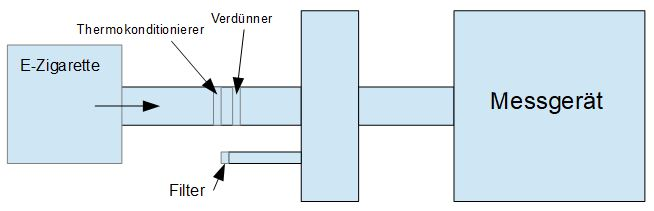
\includegraphics[width=.9\linewidth]{gfx/concepts/Konzept_5.jpg}} \quad
        \caption[Skizze Konzept 5]
        {Skizze Konzept 5}
        \label{fig:concept_5}
\end{figure}

\subsection{Funktionsweise}
Wie bei Konzept vier saugt das Messger\"{a}t in der ersten Phase gereinigte Umgebungsluft. So kann sich das Messger\"{a}t zun\"{a}chst einstellen und eine Nullz\"{a}hlrate durchf\"{u}hren. Die Schaltvorrichtung befindet sich zu Beginn in \textit{Stellung 0}. W\"{a}hrend der Nullz\"{a}hlrate des Messger\"{a}tes wird der Aerosolstrom durch den am Schaltsystem angeschlossenen Ventilator aufgebaut. Somit ist der Strom bereits geschwindigkeitsbehaftet, wenn dieser zu Messger\"{a}t umgeleitet wird. Da die Partikelanzahlkonzentration zu gro{\ss} f\"{u}r die Messger\"{a}te ist, durchstr\"{o}mt der Volumenstrom zun\"{a}chst einen Rotationsverd\"{u}nner, wo dem Aerosol gereinigte Luft beigemischt wird. Die Kombination aus Verd\"{u}nner und Thermokonditionierer arbeitet analog zu der Anwendung in Konzept vier. Anschlie{\ss}end gelangt der Volumenstrom zum Schaltsystem der Versuchseinrichtung.
\\\\
Zu einer fest eingestellten Zeit wird der Schaltmechanismus in \textit{Stellung 1} geschaltet. Dadurch str\"{o}mt das Aerosol zum Einlass des Messger\"{a}tes und erzeugt dort den Partikelsprung. Die Luftzufuhr zum Messger\"{a}t ist nun unterbrochen. Das abwechselnde Beaufschlagen von gefilterter Umgebungsluft und Aerosol gew\"{a}hrleistet einen ausreichenden Konzentrationsunterschied, um das generierte Sprungsignal zu verst\"{a}rken\cite{auswertemethodik}. Um bei Konzept vier die Totzeit des Systems so gering wie m\"{o}glich zu halten, wird der Verbindungsschlauch von Schaltsystem zu Messger\"{a}teeingang sehr kurz gew\"{a}hlt.